\section{概念、理论和方法}
\subsection{机器学习}
人工智能系统需要自己获取知识的能力,即从原始数据中提取模式(特征)的能力,这种能力称为{\Heiti 机器学习}。根据学习过程的不同经验,机器学习算法可以大致分类为监督学习算法和无监督学习算法\cite{DL, 机器学习实战}。

监督学习以含有很多特征的数据集作为训练数据,不过数据集中的每一个样本都有一个{\Heiti 标签}或{\Heiti 目标}\cite{DL}。例如,后文我们用来训练卷积神经网络模型的数据集中的每个样本都注明了它属于哪个类别。监督学习算法通过提取训练数据集中图像的特征,并分析特征与标签信息之间的对应关系,学习如何根据测量结果(提取到的特征)将样本划分为两个不同的类别。

无监督学习算法从含有很多特征的数据集中学习该数据集上有用的结构性质,而且,这种学习是在没有人为指导或注释的情况下进行的。也就是说,无监督学习一般用于从未经标注的样本分布中抽取信息\cite{DL}。例如,在后文中,我们应用了$k$-均值聚类和t-SNE这两个无监督学习算法,来从我们的数据集中抽取某种特征,而不需要借助于样本的标注信息。

\subsection{在活性物质中研究中使用机器学习}
在过去的七十年,对生物系统的理解促使机器学习算法在公式化和效率上得到了极大的提升\cite{MLAM}。同时,对机器学习的研究,也促进了认知科学、脑科学等学科的发展,同时增进了人类对自身的认识\cite{DL}。此外,大数据的发展,促进了机器学习的应用实践。作为一门数据驱动的技术,机器学习已经在许多领域得到广泛的应用。活性物质体系的复杂性,很容易让人联想到机器学习中的“维数灾难”\cite{DL, MLPM}。那么,如何将机器学习技术应用到活性物质的研究过程中呢?

事实上,机器学习技术已经被成功地应用到活性物质数据的处理中了——例如,深度神经网络用于分析图像和跟踪目标,循环网络和随机森林用于分析时间序列。此外,机器学习还可以用来帮助解开生物活性物质的复杂性,例如建立基因编码与涌现的细菌行为之间的关系,以及发现动物行为的物理线索。机器学习在活性物质研究中最重要也最常见的用途是使用监督学习算法对实验数据进行分析和分类\cite{MLAM}。计算机模拟活性物质系统的演化过程和在活性物质实验中产生的大量数据是在该领域应用机器学习的重要条件。在活性物质研究过程中应用机器学习技术可谓有得天独厚的条件。

监督学习模型通常是基于神经网络的,神经网络由大量非线性计算单元(人工神经元)通过不同权值连接构成。基于神经网络的机器学习正在成为一种强大的工具,在使用局部平衡序参数的传统回归方案不可用时(如在局域化的多体系统(MBL)或拓扑相中)获取相图\cite{PhysRevLett.120.257204}。基于卷积神经网络的监督学习甚至可以通过提高空间分辨率、扩大视野深度以及保持物体处于聚焦状态来提高活性物质实验中使用的视频显微技术。半监督学习可以利用时间序列数据来建立时空动力学的数值模型,用以解决致密活性物质在中观和宏观尺度上出现的时空模式难以用第一性原理来描述、理解和预测的问题。此外,可以利用遗传算法通过符号回归从时间序列数据中推断出潜在的模型\cite{MLAM}。

获取高维的时间序列数据背后的模型的一个有效的方法是通过投影对数据进行降维,也就是要找到一个低维的容易处理和分析的代理模型\cite{MLAM, MLPM}。在这方面,利用t-SNE(t分布随机近邻嵌入)\cite{JMLR}对数据进行降维处理是一个很好的选择。强化学习算法可以用来为船只寻找到达目标海域的最佳导航策略,同样可以用来对典型的活性物质体系的一些行为做基本的了解\cite{MLAM},如:鸟类如何在湍流气流引导的上升气流中翱翔,鱼群如何在复杂的海洋环境中穿行和聚集。


\section{数值实验的设计、目标和可行性分析}
我们的数据集是计算机模拟活性物质体系演化的过程产生的图像数据\cite{shi20180702},其中包含两类不同的图像:Polar Cluster和Percolating Turb.。后文为了方便,分别以PC和PT代之。我们希望,通过在这些数据上进行一些机器学习的数值实验,探究机器学习在活性物质研究中的应用价值。
\begin{figure}[H]
	\centering
	\subfigure[Polar Cluster]{
		\begin{minipage}[b]{0.40\textwidth}
			\centering
			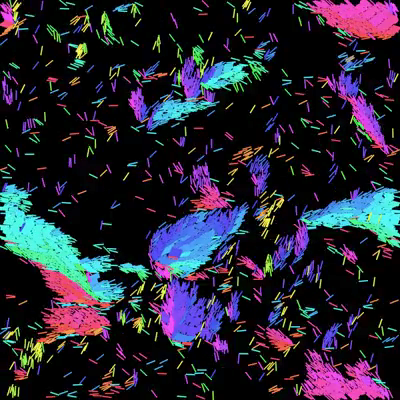
\includegraphics[width=\linewidth]{../figures/PC.png}
		\end{minipage}
		\label{fig:pc}
	}
	\subfigure[Percolating Turb.]{
		\begin{minipage}[b]{0.40\textwidth}
			\centering
			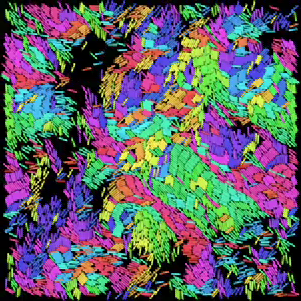
\includegraphics[width=\linewidth]{../figures/PT.png}
		\end{minipage}
		\label{fig:pt}
	}
	\caption{\textbf{本文使用的图像样本示例}:图(a)来自于PC,图(b)来自于PT。}
	\label{fig:ms}
\end{figure}

\subsection{数值实验的设计和目标}
我们的数据集一共包含$507$张图像,其中有PC图像$226$张,PT图像$281$张。我们把这些数据分为(随机采样)两个数据集合:训练集和测试集(或验证集),其中训练集中含有$45$张PC图像,$56$张PT图像,占总数据集的$20\%$,其余$80\%$包括$181$张PC图像和$225$张PT图像,作为测试集。利用这些数据,我们将进行如下4类数值实验:

1. 训练卷积网络对图像进行分类。对数据进行分类整理是从数据中发现规律的重要方法之一。我们希望,通过这次实验,探究卷积神经网络对在活性物质研究中产生的数据进行分类和识别的能力。

2. 数据的降维和可视化显示。数据可视化一直是物理研究中必备的数据分析方法,然而对于高维度的数据(如对活性物质系统演化过程进行计算机模拟生成的图像集合),直接在二维和三维的坐标系中进行可视化并不现实,因此我们想通过这次实验,探究对高维数据进行可视化的方法及效果。

3. 识别数据集中有多少种数据。我们希望通过对数据集进行无监督学习,探究能否利用机器学习,直接对没有标注信息的原生数据进行分析,比如:识别出数据的类别数目,以及将数据进行分组整理。

4. 从指定数据集中检索和提取与输入图像同类图像,类似于“以图搜图”。提高数据检索和提取的效率对于提高科研效率有着极大的帮助,我们希望,通过这次实验,探究构造一个搜索同类数据的系统的可能性。

\subsection{可行性分析}
我们选择了Python语言作为我们进行数值实验的工具。Python语言简洁易用,能够快速上手,拥有很多开源库支持,在很大程度上降低了实验的难度。此外,我们已经有了进行我们的数值实验必不可少的材料——活性物质研究中的数据。因此,我们的实验具备可行性。


\section{数值实验的过程及结果分析}
\subsection{利用卷积网络对图像进行分类}
卷积网络,又称卷积神经网络(Convolutional Neural Network, CNN),是一种专门用于处理具有类似网络结构的数据的计算模型\cite{DL}。卷积网络在许多领域都表现优异,尤其是在计算机视觉领域,人们常用它来提取图像的特征,以进行图像分类、识别和检索等任务。

%人工神经网络是机器学习中联结主义的产物,网络一般由许多层通过不同的权值连接而成。卷积神经网络指至少含有一个卷积层的神经网络
卷积神经网络是一种监督学习方法,其学习(训练)过程有点类似于人的学习过程:对数据应用一种处理方法,得出一个结果;$\Rightarrow$ 对结果与目标之间的误差进行分析;$\Rightarrow$ 反馈出现误差的原因;$\Rightarrow$ 根据原因改进方法。具体体现在卷积神经网络模型的训练步骤上为:

1. 初始化模型参数;

2. 将数据代入模型得出结果;

3. 运用损失函数(在机器学习中,损失函数、代价函数和误差函数是同义词\cite{DL})计算结果与目标之间的误差;

4. 通过链式法则将误差对权值的导数向后传递至网络各层,这一步又称作对误差进行反向传播\cite{DL};

5. 根据误差对各层权值的导数,运用优化器对模型进行改进;

第2\textasciitilde 5步叫做一个训练循环,一般会进行多次,直到得到一个满意的模型。总的来说,卷积神经网络的训练过程大致是一个运用梯度下降算法\cite{DL}对损失函数进行最小化的过程。

\subsubsection{构建实验模型}\label{vgg16model}
在该实验中,我们借助PyTorch\cite{DLWP}构建了一个如图\ref{fig:vgg16}所示的VGG16模型\cite{vgg16},用交叉熵损失函数\cite{DL, DLWP}计算训练误差并进行反向传播,用Adam优化器\cite{DL, DLWP}对模型参数进行优化。交叉熵损失函数的公式如下
\begin{equation}\label{equ:CrossEntropyErrorFunction}
L=\frac{1}{N} \sum_{i}^{N} L_{i}=\frac{1}{N} \sum_{i}^{N} -\left[y_{i} \cdot \log \left(p_{i}\right)+\left(1-y_{i}\right) \cdot \log \left(1-p_{i}\right)\right]
\end{equation}
其中$y_i$表示样本$i$的类别标签,$p_i$表示样本$i$预测为$y_i$的概率。$N$为输入样本的个数,这里是对所有样本取平均。

\begin{figure}[H]
	\centering
	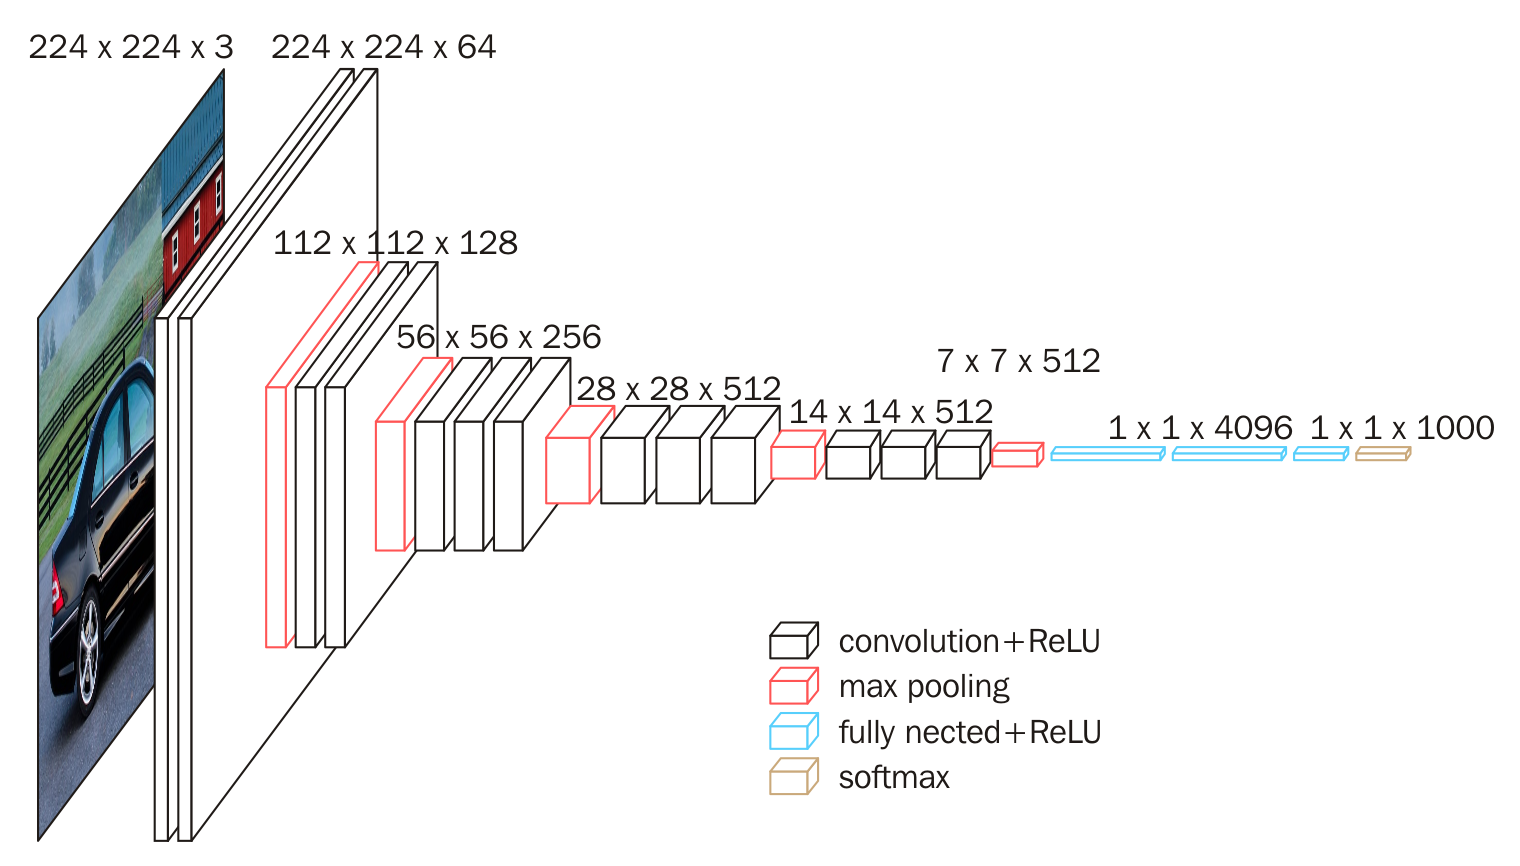
\includegraphics[width=0.8\linewidth]{../figures/vgg16.png}
	\caption{\textbf{VGG16模型的结构图}:模型以一张$224 \times 224 \times 3$的图像作为输入,输出一个一维张量,表示对图像的预测为各个类别的概率。}
	\label{fig:vgg16}
\end{figure}

在使用过程中,图像首先被加载进入内存并缩放到$224 \times 224 \times 3$大小,然后转化为PyTorch三维张量(Tensor)\cite{DLWP}并经过标准化处理,使其中的每个数值处于$[-1, 1]$这个范围。为了效率上的提升,图像是一批一批地输入模型,在GPU上并行计算的。因此,我们的模型实际上是以一个四维张量作为输入。经过网络的层层计算和转化,模型最终输出一个二维张量,其行数与输入图像的张数相等,每一行有$m$(预设的类别数目)个元素,每个元素$p_i$表示代表该行对应的图像属于第$i$个类别的概率。

对于模型输出的二维张量,我们计算每一行中的最大概率所在的列的标号,然后以之作为索引,到存有类别名称的数组中去获取对应的图像的预测分类。

下面是一个简单的例子

假设我们给模型预设了3个类别,类别名称分别为cat, dog, desk并按顺序存于数组C中,因此C = [cat, dog, desk]。对于已经转化好的图像[img1, img2],模型的输出是
\begin{equation*}\label{equ:example}
	\begin{bmatrix}
		0.5 & {\color{red} 0.8} & 0.2\\
		0.3 & 0.5 & {\color{red} 0.9}
	\end{bmatrix}
\end{equation*}
那么,计算每一行中最大概率所在的列的标号,我们会得到一个含有两个元素的数组:[2, 3]。然后,以数组中的每个元素作为索引到类别名称数组C中去获取对于的类别名称,我们就得到了预测的分类:img1属于dog,img2属于desk。

\subsubsection{数值实验的过程简述}
在实验过程中,为了防止过拟合\cite{DL, DLWP},训练集数据以乱序进入模型;测试集的数据用于测试模型是否过拟合,并验证经过训练后的模型是否具有识别训练集之外的数据的能力(泛化能力)。另外,为了不必每次使用模型时都得重新训练,减少不必要的漫长等待,以及防止突然的机器故障,在每一轮训练循环之后,程序都会将模型的参数保存到硬盘。每一次保存都会将上一次保存的参数覆盖,但是最好的参数(对测试集进行分类的正确率最高)会被另存一份。

最初,我们以80\%的数据作为训练集,20\%的数据作为测试集。检查训练过程中的正确率和误差,我们发现,测试集的表现居然比训练集还要好。我们以为是因为测试集数据量较少的缘故,于是互换了测试集和训练集,发现依然如故——模型在测试集上的正确率和误差均比在训练集上的要好并且稳定,如图\ref{fig:c1}。一时间百思不得其解,经查阅资料发现,这是因为我们在训练过程中开启的是train模式\cite{DLWP},而在测试过程中开启的是eval(评估)模式\cite{DLWP}。在train模式下,模型中的Dropou层\cite{DL}会被打开,该层以50\%的概率扔弃掉上一层输入的数据,以防止过拟合,于是模型在训练集上的正确率就变得偏低并且不稳定。在实际工作中使用模型时,Dropout层是要关闭的。

重新在训练集上开启eval模式进行测试的结果表明:模型在训练集上的结果确实要比在测试集上的略好,如图\ref{fig:c2},这才是与理论相符的结果。

最后,我们用经过预训练的VGG16模型进行迁移学习\cite{DL},发现其具有强大的学习能力,仅需一次学习,就能够以$100\%$的正确率完全识别我们的训练集和测试集。如图\ref{fig:c3}

\subsubsection{数值实验结果展示及分析}
\begin{figure}[H]
	\centering
	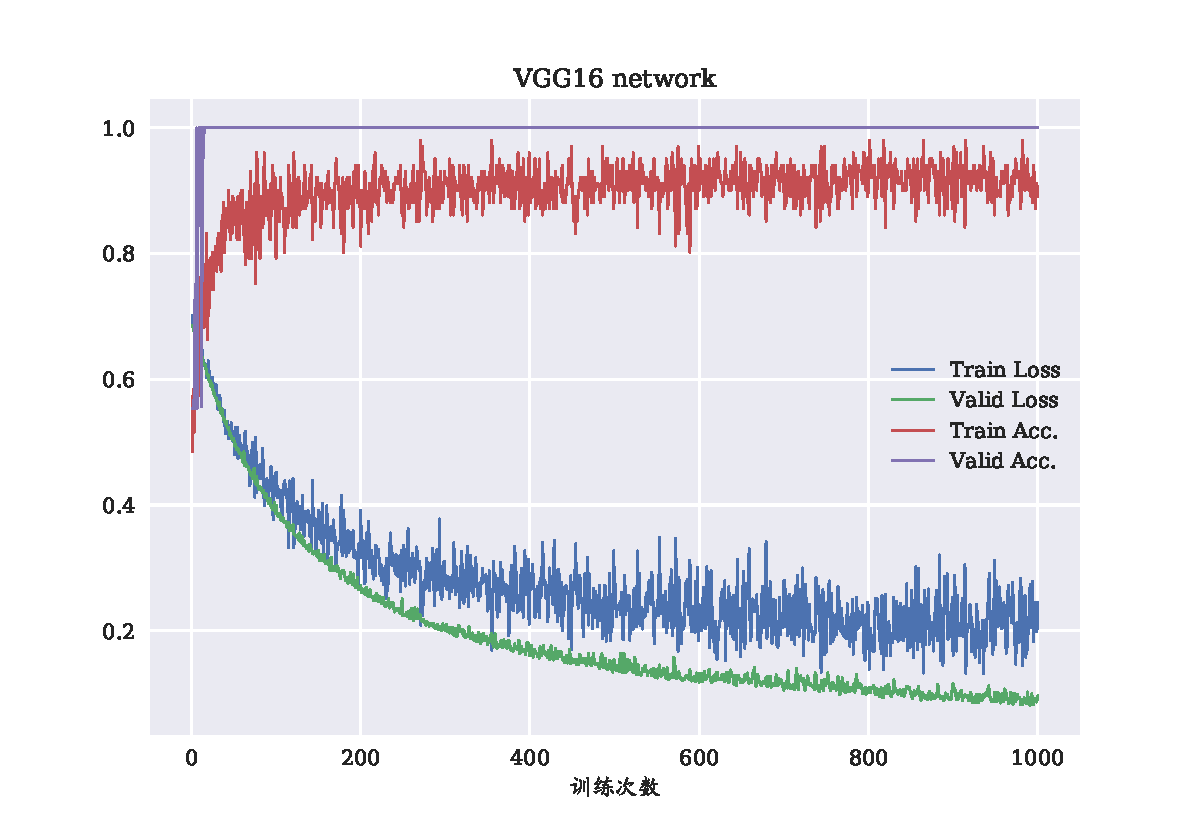
\includegraphics[width=\linewidth]{../figures/classifier/1.pdf}
	\caption{\textbf{模型训练过程中正确率和误差变化趋势}:Train Loss和Valid Loss分别代表训练集上的误差和测试集上的误差,Train Acc.和Valid Acc.分别代表训练集上的正确率和测试集上的正确率。图中没有对训练集额外进行与测试集同样的测试,训练集的测试结果直接取自训练过程,因此对训练集的测试相当于是在开启Dropout层的情况下进行的,所以看起来没有测试集的好。}
	\label{fig:c1}
\end{figure}

\begin{figure}[H]
	\centering
	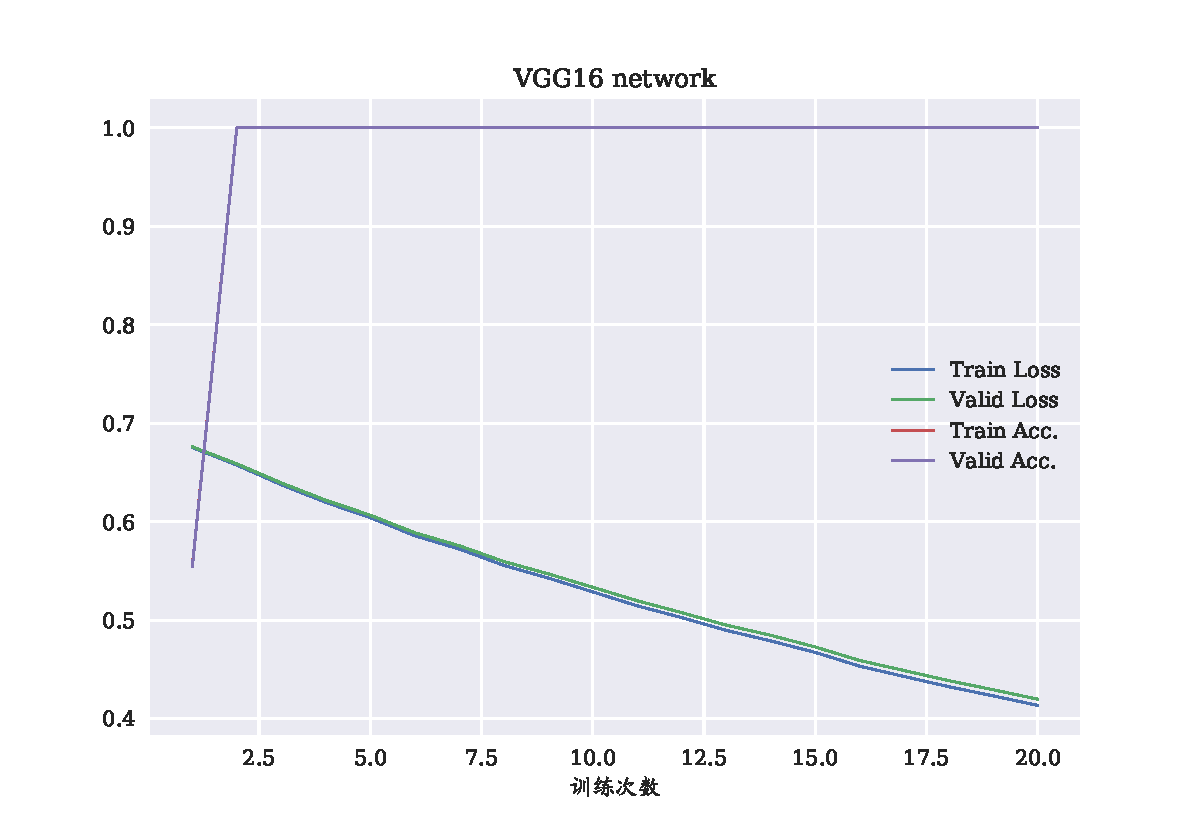
\includegraphics[width=0.95\linewidth]{../figures/classifier/2.pdf}
	\caption{\textbf{模型训练过程中正确率和误差变化趋势}:同上图,但是对训练集做了和测试集同样的测试,因此训练集上的结果相比测试集上的略好。}
	\label{fig:c2}
\end{figure}

\begin{figure}[H]
	\centering
	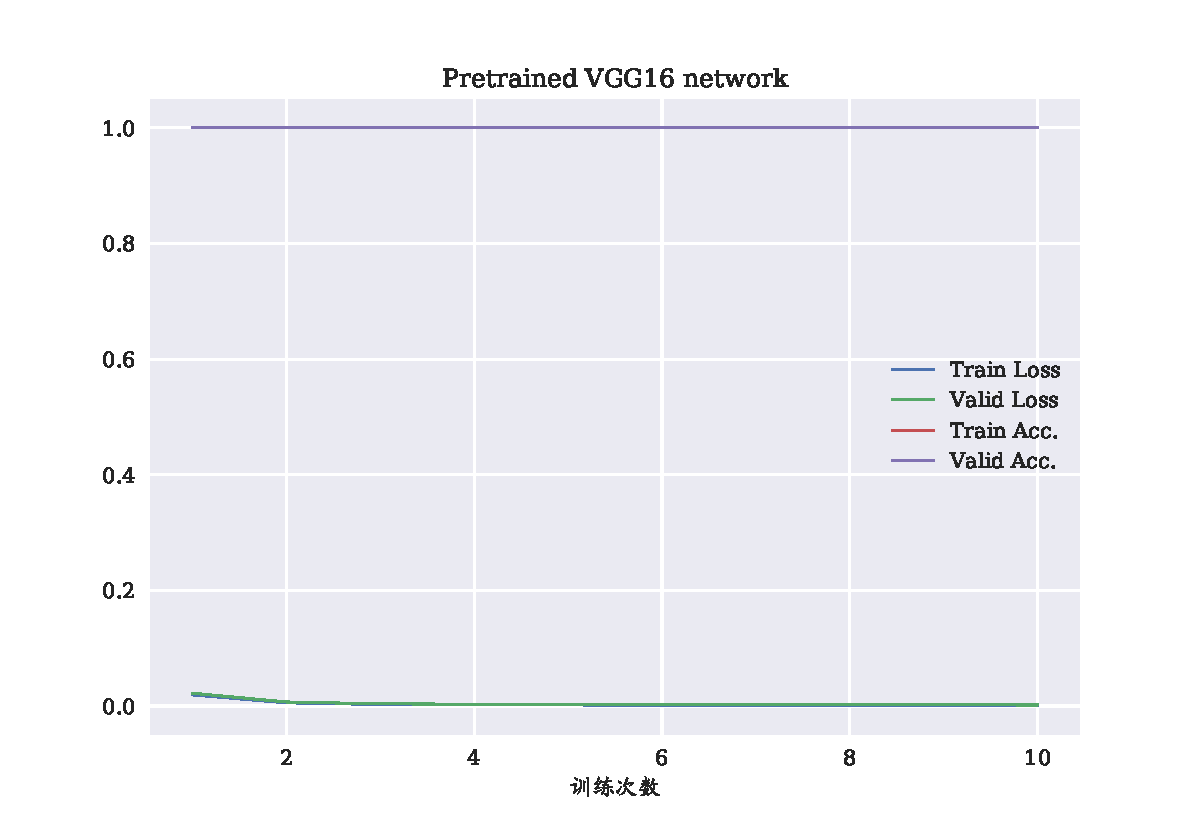
\includegraphics[width=0.95\linewidth]{../figures/classifier/3.pdf}
	\caption{\textbf{用经过预训练的VGG16模型进行迁移学习时正确率和误差变化趋势}:可以看到,经过一次学习后,识别率就达到了100\%。}
	\label{fig:c3}
\end{figure}

\begin{figure}[H]
	\centering
	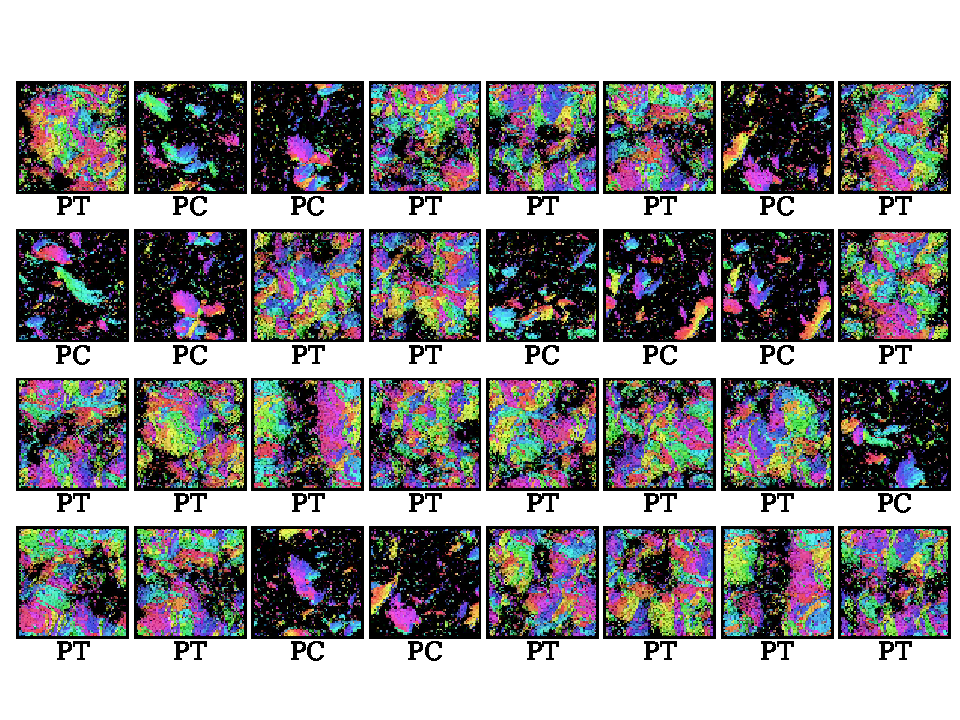
\includegraphics[width=\linewidth]{../figures/classifier/示例.pdf}
	\caption{\textbf{图像识别示例}:经过训练之后的模型对测试集中随机选取的32张图像进行识别,每张图像下面展示了模型对该图像进行预测的结果。}
	\label{fig:cexample}
\end{figure}

迁移学习是一种跨领域适应的学习能力\cite{DL}。比如,我们可以将自己学过的数学知识应用到对物理学的学习中,从而提高物理学习效率。

我们的实验结果表明,卷积神经网络对于识别和分类活性物质研究中的图像有着巨大的潜力,尤其是对具有很强的自适应能力的网络(如VGG16),利用迁移学习方法,可以有效地提高训练效率,减轻计算机的运算负担和能源消耗。

\subsection{数据的降维和可视化显示}
受思维和空间的双重限制,我们无法将维数超过三维的数据集(比如一批高清的图像)在坐标轴上用一个一个的坐标点标记出来,从而不能对数据点之间的位置关系和距离有着直观的理解。T分布随机近邻嵌入(\textrm{T-Distribution Stochastic neighbour Embedding, t-SNE})\cite{JMLR}为我们提供了这种可能。t-SNE是一种常用的数据降维算法,同时也是一种数据压缩算法,它的作用是在保留原有数据点之间的邻居关系的同时,把数据点从高维特征空间映射到二维或三维空间,是一种无监督学习算法\cite{DL}。

对于我们的图像数据集,我们利用了t-SNE算法将其降维到二维和三维并以不同的颜色绘制了出来,如图\ref{fig:tsne},图中每一个点代表一张图像。

\begin{figure}[H]
	\centering
	\includegraphics[width=\linewidth]{../figures/TSNE/tsne可视化.pdf}
	\caption{\textbf{本文所使用的图像集的t-SNE可视化显示。}图中展示了通过t-SNE算法将我们的图像集降维到2维和3维后的坐标点之间的邻居关系。}
	\label{fig:tsne}
\end{figure}

通过对不同类别的图像使用不同的颜色进行标记,可以清晰的看到,t-SNE降维保持了样本点之间的邻居关系。同类图像在二维和三维空间中依然簇拥在一起,不同类别的图像之间则泾渭分明。

\subsection{识别数据集中有多少种数据}
\subsubsection{对图像进行$k$-均值聚类}
分类适用于我们知道类别属性的数据,而对我们原本不知道类别信息的数据,聚类是一种对数据进行预处理的重要手段。聚类是常用的无监督学习方法,主要被运用来处理未经标注的数据。数据科学教们已探索出许多高效的聚类算法,其中最常用也最容易实现的是$k$-均值聚类算法\cite{DL, 机器学习实战}。$k$-均值算法从数据点中选取$k$个点作为质心(聚类中心),然后围绕这$k$个质心按照最小距离(欧氏距离\ref{equ:EuclideanDistance})原则将数据点划分为$k$个簇,然后再以每个簇中数据点的平均值作为新的质心。后两步会进行多次,直到质心不再发生变化。那么,如何对图像进行$k$-均值聚类?

$k$均值算法原理简单,我们直接调用了sklearn库\cite{sklearn}中的实现。需要注意的是,sklearn库中对$k$均值算法的实现以$k$值和一个不高于二维的numpy\cite{numpy}数组作为输入。因此,我们可以对经过t-SNE降维后的坐标点集合进行聚类,或者对CNN提取的图像特征(线性层的输出)集合进行聚类,这两者都是二维矩阵,每一行代表一张图像。此外,在我们的数值实验中,我们使用了另外一种方法。我们先对每张图像进行了缩放和灰度处理,然后转换为numpy数组并展平到一维,所有图像组合成为一个numpy二维数组,作为$k$-均值算法的输入。最后,$k$-均值算法会输出聚类结果,其中包括$k$个质心的坐标,以及每一个数据点所属的簇的编号($1\textasciitilde k$)。

\subsubsection{利用SSE-$k$曲线找到最优聚类}
由于$k$-均值算法需要$k$值作为输入,因此其并不能直接告诉我们一个数据集应该聚类成为几个簇。事实上,根据不同的要求,我们可以把一个数据集划分成$1\textasciitilde n$个组,其中$n$是该数据集中数据点的个数。因此,我们需要一种方法来从$n$个值中找出最佳的聚类数目,从而识别数据集中有多少种数据。

SSE(Sum of the Squared Errors, 误差平方和)是一种衡量聚类效果的方法\cite{机器学习实战},其代表的是所有数据点到其对应的聚类中心的距离之和:
\begin{equation}\label{equ:sse}
SSE = \sum_{i=1}^{k}\sum_{p\in C_i}|p-m_i|^2
\end{equation}
其中$C_i$表示第$i$个簇,$p$是$C_i$中的数据点,$m_i$是$C_i$的质心。

如图\ref{fig:cluster},我们展示了以不同$k$值对我们的数据集进行聚类的SSE值——$SSE-k$曲线。可以看到,随着$k$的增大,SSE逐渐减小。而且,当$k$小于真实的类别数目时,SSE的下降得很快,当$k$超过真实的类别数目后,SSE下降迅速减缓。这是因为,随着质心个数的增加,簇就会越来越小,簇中的数据点离质心就会越来越近,因而SSE逐渐变小。极端情况就是当$k$增加到$n$时,结果中有$n$个簇,每个簇中仅一个元素,每个元素都是质心,这时SSE等于0。当$k$值从1增加到等于真实的类别数目后,增加$k$值不过是将本该属于同一个类别的数据点再进行划分,并且越往后面,簇越小,簇分裂产生的两个簇之间离得越近,对SSE的影响就越小。

\begin{figure}[H]
	\centering
	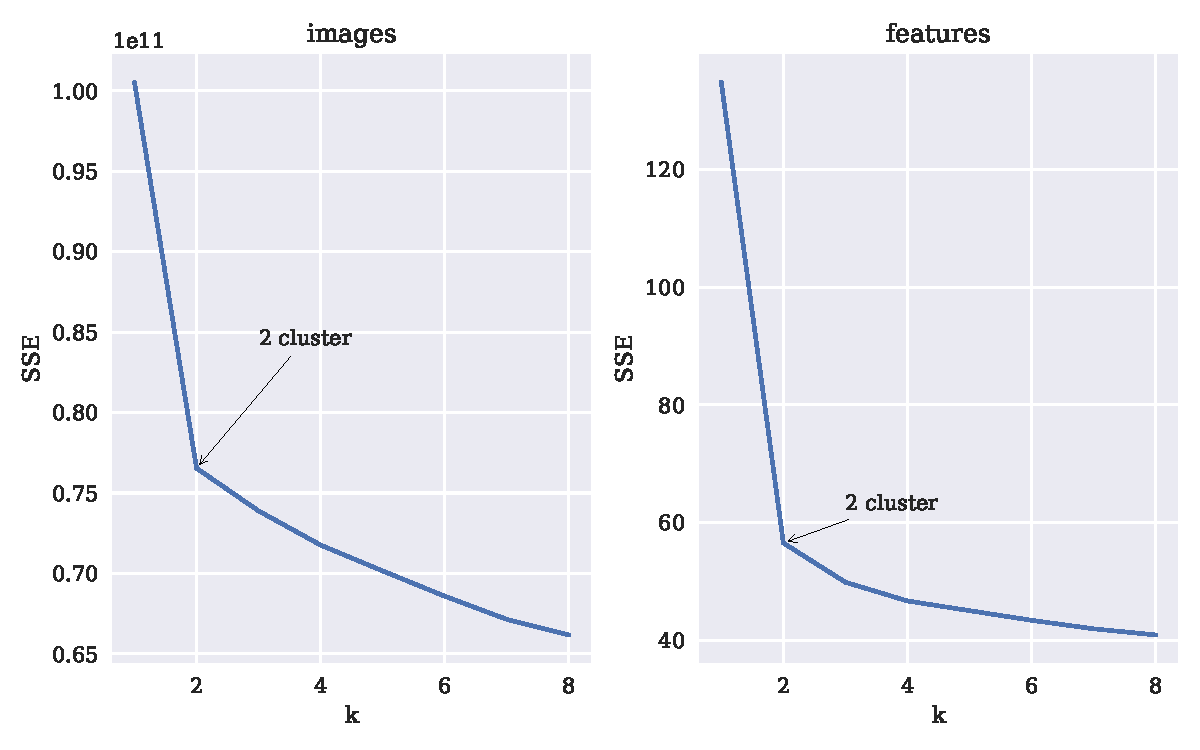
\includegraphics[width=\linewidth]{../figures/cluster/1.pdf}
	\caption{\textbf{利用SSE-$k$曲线确定最好的聚类数目。}图中显示了以不同$k$值进行聚类计算得到的SSE。左图以图像作为输入,右图以CNN提取的图像特征作为输入。}
	\label{fig:cluster}
\end{figure}

对于我们的数据集,$SSE-k$曲线在$k$增到2时出现了一个大的转折点,这是因为我们的数据中有PC和PT两种图像,符合上面的分析。因此,通过分析$k$-均值聚类的$SSE-k$曲线,可以有效地识别出数据集中数据类别的数目。

\subsection{从图像集合中检索和提取同类图像}
数据检索的目的在于,通过输入已知的部分数据,我们可以从数据库中检索和提取我们所需的相似样本。数据检索分为从数据库中检索和从原始数据中检索,从数据库中检索信息需要有一个已经整理好的数据库,不在本文研究范围。本文研究的是从未经分类整理的原始数据集中检索与输入的图像属于同一类别的图像,属于一种无监督学习方法:算法对输入的图像进行学习,然后到一个指定的数据集中去寻找与之相似的图像。为此,我们从上述分类实验的训练集(20\%)中选取一类图像的部分或全部给模型进行无监督学习,然后让其从打乱后的测试集(80\%)中检索同类图像。当以多张图像作为输入时,输入的是图像的平均值。

在数值实验过程中,我们记录了每个样本的类别,类别并不会被用来辅助检索,但是会被用于计算检索结果的正确率和误差。我们实验了两类不同的方法:一类是通过相似度进行检索,另一类通过距离进行检索。这里的相似度和距离并没有严格的定义,只是一个表征的数值。

\subsubsection{通过样本相似度进行检索}
通过相似度进行图像检索的具体步骤是:

1. 计算出输入的图像与测试集中每张图像的相似度;

2. 按照相似度降序排列图像,并使用一个阈值截掉部分图像(扔掉相似度小于某个值的图像);

3. 利用差分运算找到第一个相似度断崖式下降的点,作为{\Heiti 分界线};

4. 将分界线左边的样本输出,作为检索的结果。

我们使用了余弦相似度公式来计算图像的相似度,余弦相似度的计算公式如下
\begin{equation}\label{equ:CosineSimilarity}
S = \frac{A \cdot B}{\Vert A\Vert \Vert B \Vert} = \frac{\sum\limits_{i=1}^{n} A_i \times B_i}{\sqrt{\sum\limits_{i=1}^{n} (A_i)^2} \times \sqrt{\sum\limits_{i=1}^{n} (B_i)^2}}
\end{equation}
其中$A$, $B$是一维张量,代表要计算相似度的两张图像。

为了使图像能够作为余弦相似度函数的输入,我们需要把每张图像转换成为一维张量。其中最直接也最简单的一个方法是,直接将每张图像展平成为一位张量。但是,我们通过实验发现这种方法不具备可行性,如图\ref{fig:rcs}。

\begin{figure}[H]
	\centering
	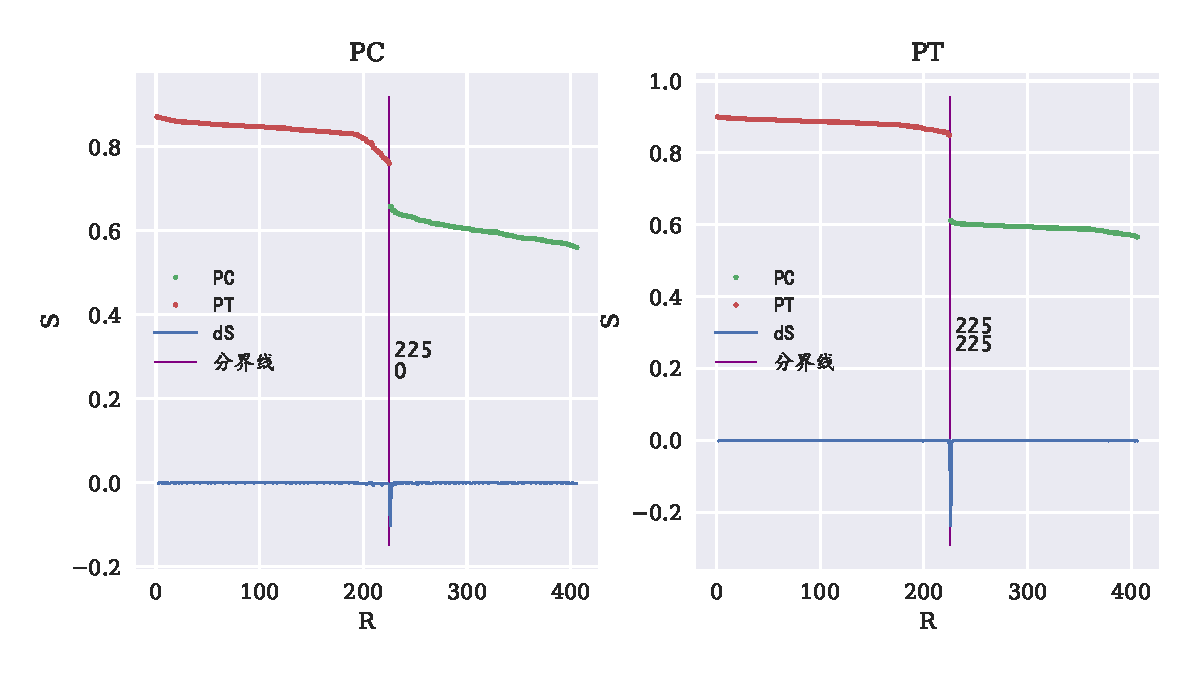
\includegraphics[width=\linewidth]{../figures/retrieval/2.pdf}
	\caption{\textbf{通过图像的余弦相似度进行图像检索}:左图以PC图像作为输入,右图以PT图像作为输入。其中R表示相似度排名,S为相似度,dS是S的变化量。分界线右侧的两个数字分别是检出图像数和检出图像正确数,这些数字显示,无论输入PC图像还是输入PT图像,检索出来的都是PT图像。}
	\label{fig:rcs}
\end{figure}

为了证实不是由于数值实验过程中出现错误导致了上述结论,我们随机抽取了四张图像(PC和PT各两张),分别命名为PC1, PC2, PT1, PT2,如图\ref{fig:cs}。然后用上述方法计算了它们之中不同图像的相似度,如下表。

\begin{figure}[H]
	\begin{minipage} [b]{.45\linewidth}
		\centering
		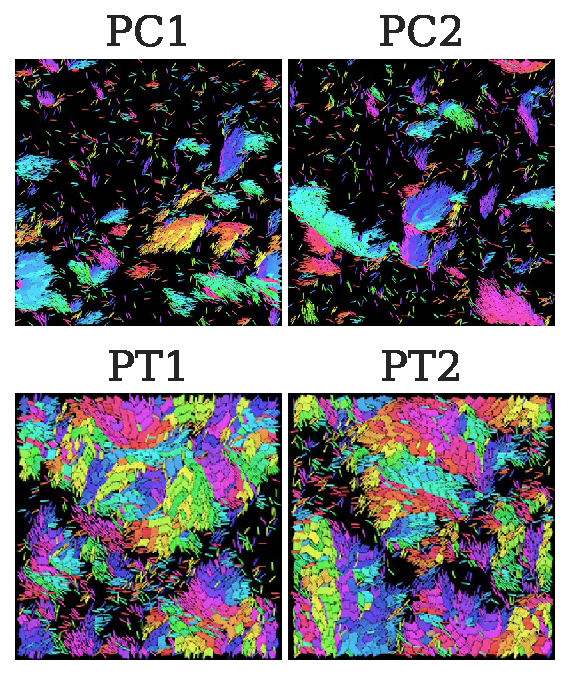
\includegraphics[width=3.8cm]{../figures/retrieval/PCPT.pdf}
		\caption{输入图像}\label{fig:cs}
	\end{minipage}
	\begin{minipage} [b]{.55\linewidth}
		\begin{tabular}{C{3cm}|L{3cm}}
			\hline
			输入图像 & \hspace{1.8em}相似度 \\
			\hline
			PC1 vs. PC1 & \hspace{2em}1.0\\
			PC1 vs. PC2 & \hspace{2em}0.3475\\
			PC1 vs. PT1 & \hspace{2em}0.4725\\
			PC1 vs. PT2 & \hspace{2em}0.5192\\
			PT1 vs. PT2 & \hspace{2em}0.7989\\
			PT1 vs. PC2 & \hspace{2em}0.5287\\
			PT2 vs. PC2	& \hspace{2em}0.5820\\
			\hline
		\end{tabular}
		\captionsetup{type=table}
		\label{table:cs}
		\caption{输入图像的相似度}
	\end{minipage}
\end{figure}
可以看到,PT1与PT2的相似度最高,而PC1与PC2的相似度最低,PC1与PT1的相似度(0.4725)比PC1与PC2的相似度(0.3475)还高。因此,输入PC图像检索到的全是PT图像就不难理解了,这是对图\ref{fig:rcs}最好的解释。

于是我们换了一种方法:使用VGG16模型提取图像特征(如我们在\ref{vgg16model}这一小节中所说,VGG16对每张图像输出一个一维特征向量),作为余弦相似度算法的输入。下面展示的结果支撑了这一方法的可行性。

\begin{table}
	\centering
	\begin{tabular}{C{2.5cm}|C{2cm}|C{2.5cm}|C{2.5cm}|C{2.0cm}}
		\hline
		输入图像数 & 检出数 & 检出正确数 & 检出错误数 & 未检出数 \\ \hline
		\hspace{0.4em}1 & 179 & 179 & 0 & 2\\ % \hline
		\hspace{0.4em}2 & 189 & 181 & 8 & 0\\ % \hline
		\hspace{0.4em}3 & 179 & 179 & 0 & 2\\ % \hline
		\hspace{0.4em}4 & 179 & 179 & 0 & 2\\ % \hline
		\hspace{0.4em}5 & 189 & 181 & 8 & 0\\ % \hline
		10 & 177 & 177 & 0 & 4\\ % \hline
		15 & 183 & 181 & 2 & 0\\ % \hline
		20 & 181 & 181 & 0 & 0\\ % \hline
		25 & 181 & 181 & 0 & 0\\ \hline
	\end{tabular}
	\caption{PC的检索结果随输入图像张数的变化}
	\label{tab:PC}
\end{table}

\begin{table}[H]
	\centering
	\begin{tabular}{C{2.5cm}|C{2cm}|C{2.5cm}|C{2.5cm}|C{2.0cm}}
		\hline
		输入图像数 & 检出数 & 检出正确数 & 检出错误数 & 未检出数 \\ \hline
		\hspace{0.4em} 1 & 401 & 225 & 176 & 0\\ % \hline
		\hspace{0.4em} 2 & 227 & 225 & 2 & 0\\ % \hline
		\hspace{0.4em} 3 & 227 & 225 & 2 & 0\\ % \hline
		\hspace{0.4em} 4 & 225 & 225 & 0 & 0\\ % \hline
		\hspace{0.4em} 5 & 225 & 225 & 0 & 0\\ % \hline
		10 & 225 & 225 & 0 & 0\\ % \hline
		15 & 225 & 225 & 0 & 0\\ % \hline
		20 & 225 & 225 & 0 & 0\\ % \hline
		25 & 225 & 225 & 0 & 0\\ \hline
	\end{tabular}
	\caption{PT的检索结果随输入图像张数的变化}
	\label{tab:PT}
\end{table}

表\ref{tab:PC}和表\ref{tab:PT}展示了检索的结果随输入图像张数的变化。其中的结果表明:随着输入图像的增加,检索的效果会越好。

\begin{figure}[H]
	\centering
	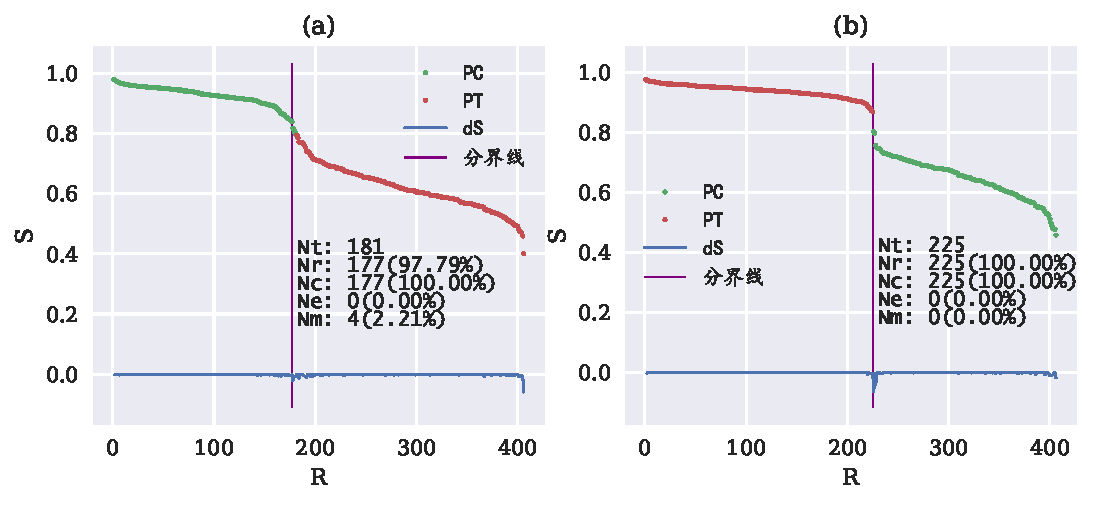
\includegraphics[width=\linewidth]{../figures/retrieval/8.pdf}
	\caption{\textbf{输入8张图像时的相似度和检索结果}:图(a),(b)分别以PC和PT作为输入。S为相似度,R为相似度排名,dS是S的变化率。分界线的右侧的五个数据分别是:Nt—测试集中同类图像总数,Nr—检出数,Nc—检出正确数,Ne—检出错误数,Nm—未检出数。}
	\label{fig:r1}
\end{figure}

\begin{figure}[H]
	\centering
	\subfigure[输入的8张图像]{
		\begin{minipage}[b]{0.18\textwidth}
			\centering
			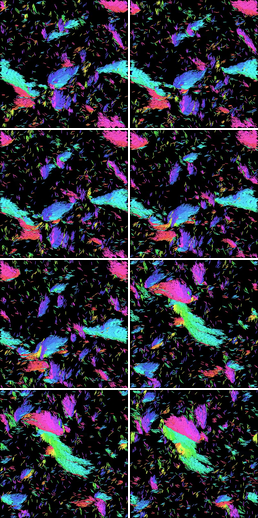
\includegraphics[width=\linewidth]{../figures/retrieval/示例input.png}
		\end{minipage}
		\label{fig:exam-input}
	}
	\subfigure[检索结果中位于分界线附近的40张图像]{
		\begin{minipage}[b]{0.72\textwidth}
			\centering
			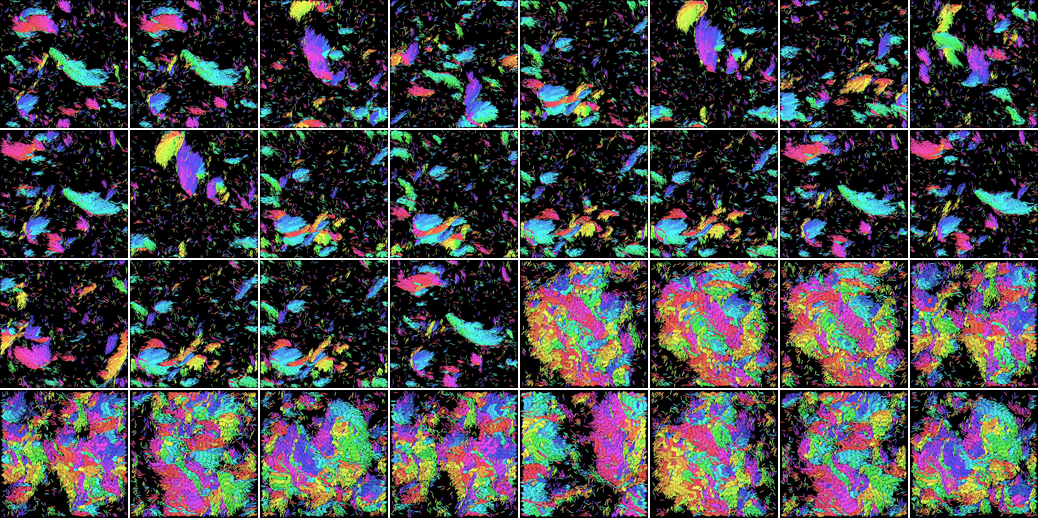
\includegraphics[width=\linewidth]{../figures/retrieval/示例output.png}
		\end{minipage}
		\label{fig:exam-output}
	}
	\caption{\textbf{检索结果展示}:图中展示了从训练集中随机选择的8张图像作为输入,到训练集中进行检索的结果。图(b)展示了相似度分界线前后各20张图像,其中有4张同类图像由于位于分界线之后,成了漏网之鱼。}
	\label{fig:example}
\end{figure}

\begin{figure}[H]
	\centering
	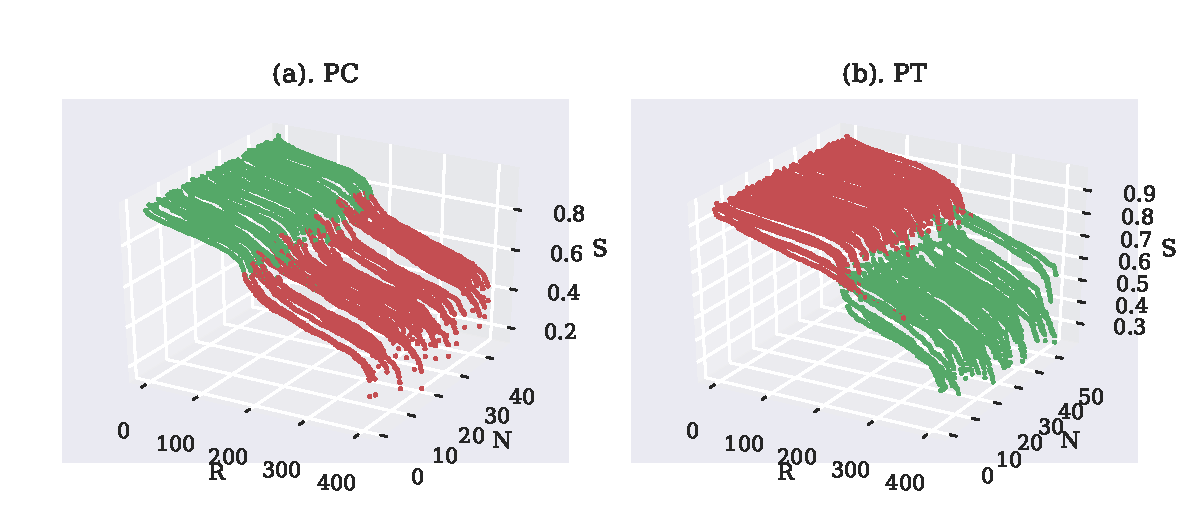
\includegraphics[width=\linewidth]{../figures/retrieval/onebyone.pdf}
	\caption{\textbf{训练集中每张图像与测试集中所有图像的相似度降序排列}:图(a),(b)分别以PC和PT作为输入。PC图像以绿点标出,PT图像以红点标出。图中轴标N, R, S分别代表输入图像的序号,排名和相似度。}
	\label{fig:r-onebyone}
\end{figure}

图\ref{fig:r-onebyone}以不同的颜色画出训练集中每张图像与测试集中所有图像的相似度的降序排列。可以看到,虽然会出现一些偏差,但总体上,同类图像的相似度排名比较靠前,异类的比较靠后,中间存在一个断崖。因此,这种相似度算法还是比较可靠的。

\subsubsection{通过样本距离进行检索}
1. 计算出输入的图像与测试集中每张图像的距离;

2. 按照距离升序排列图像,并使用一个阈值截掉部分图像(扔掉距离大于某个值的图像);

3. 利用差分运算找到第一个距离断崖式上升的点,作为{\Heiti 分界线};

4. 将分界线左边的样本输出,作为检索的结果。

我们运用了欧式距离公式来计算图像之间的距离,其表达式如下:
\begin{equation}\label{equ:EuclideanDistance}
dist(X, Y) = \sqrt{\sum\limits_{i=1}^{n} (x_i - y_i)^2}
\end{equation}
其中$X = \{x_1, x_2, \cdots, x_n\}$, $Y = \{y_1, y_2, \cdots, y_n\}$ 为两个一维张量,代表要计算距离的两个数据点。

为了使图像能够作为欧式距离算法的输入,我们使用了如下两种方法对图像进行预处理,发现它们都很有效。

1. 使用t-SNE降维算法,将图像集映射到二维平面上的点集。

2. 对每张图像进行缩放和灰度化处理(为了减少运算量),然后展平成为一个一维张量。

\begin{figure}[H]
	\centering
	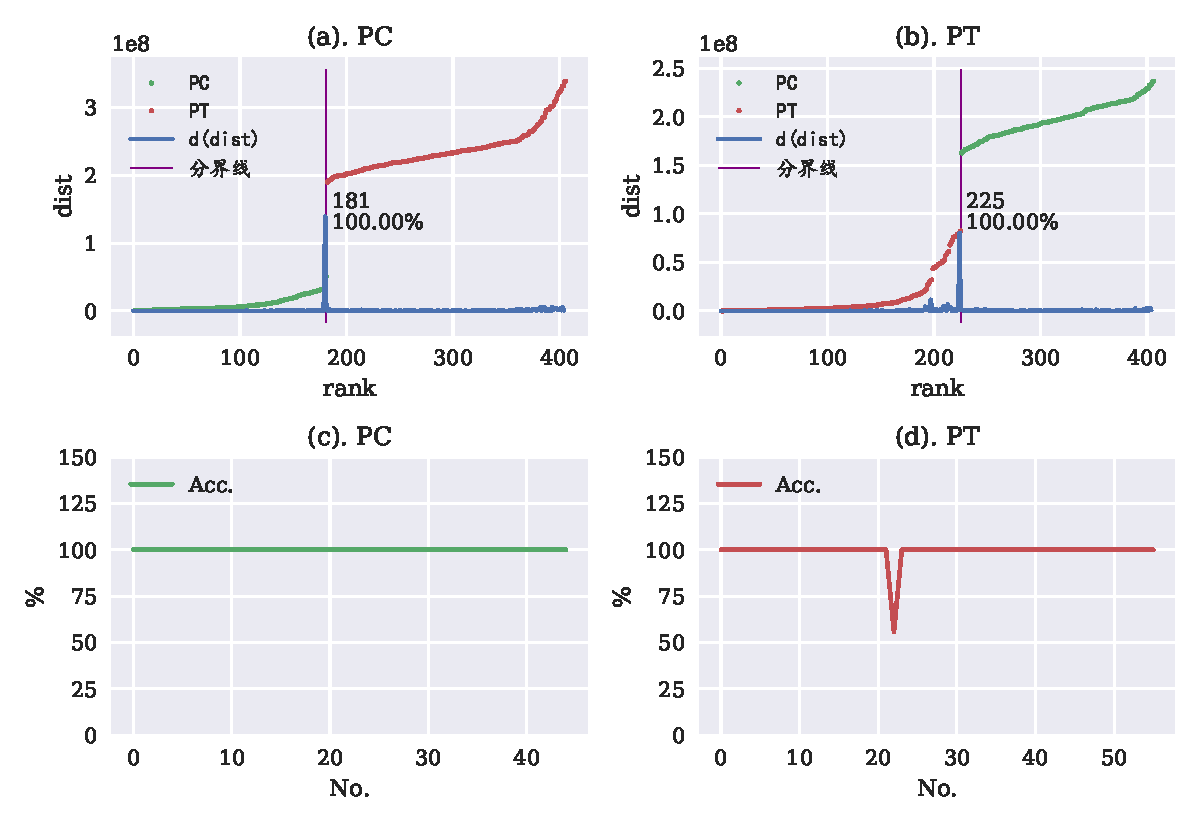
\includegraphics[width=\linewidth]{../figures/retrieval/TSNE-dist2.pdf}
	\caption{\textbf{通过样本距离检索图像}:(a), (b)分别为输入5张PC图像和5张PT图像的检索结果,其中d(dist)表示对距离做差分运算。(c), (d)展示了每次输入1张图像进行检索的正确率,分别代表PC和PT。}
	\label{fig:o1}
\end{figure}



